\documentclass[12pt,a4paper]{article}
\usepackage{cmap}
\usepackage[utf8]{inputenc}
\usepackage[T1,T2A]{fontenc}
\usepackage[english,russian]{babel}
\usepackage{array,booktabs,tabularx,amsmath}
\usepackage{caption,float,graphicx,qrcode}
\usepackage{geometry,hyperref,indentfirst,tocloft}
\geometry{margin=25mm}
\hypersetup{unicode=true,colorlinks=true,urlcolor=blue,linkcolor=black}
\setlength{\parindent}{1.25cm}
\setlength{\parskip}{0pt}
\setlength{\emergencystretch}{2em}
\setcounter{tocdepth}{2}
\setlength{\cftbeforesecskip}{5pt}
\setlength{\cftbeforesubsecskip}{1pt}
\renewcommand{\cftsecfont}{\normalsize\bfseries}
\renewcommand{\cftsecpagefont}{\normalsize\normalfont}
\renewcommand{\cftsubsecfont}{\normalsize\normalfont}
\renewcommand{\cftsubsecpagefont}{\normalsize\normalfont}
\renewcommand{\cftdotsep}{1}
\renewcommand{\labelitemi}{\textendash}
\DeclareCaptionLabelSeparator{emdash}{\space---\space}
\captionsetup[figure]{justification=centering,singlelinecheck=false,labelsep=emdash}
\addto\captionsrussian{\renewcommand{\figurename}{Рис.}}
\newcommand{\code}[1]{\texttt{\detokenize{#1}}}
\newcolumntype{P}[1]{>{\raggedright\arraybackslash}p{#1}}
\newcommand{\ReportDate}{22.10.2026}
\newcommand{\CorpusDocuments}{27\,014}
\newcommand{\CorpusMB}{85,42}
\newcommand{\TokenCount}{9\,020\,624}
\newcommand{\KnownPercent}{80,27}
\newcommand{\ChangedTokens}{3\,230\,212}
\newcommand{\AmbiguousTokens}{1\,003\,108}
\newcommand{\DictionaryEntries}{3\,111\,758}
\newcommand{\DictionaryMB}{132,99}
\newcommand{\DictionaryMemoryMB}{166,54}
\newcommand{\ProcessingMs}{6\,023,36}
\newcommand{\ElapsedMs}{6\,176,49}
\newcommand{\LoadMs}{1\,046,85}
\newcommand{\TokensPerSecond}{1\,497\,607}
\newcommand{\PoolDocuments}{37}
\newcommand{\QueryCount}{12}
\newcommand{\CppChecks}{66}
\newcommand{\PythonChecks}{17}
\newcommand{\BenchmarkRuns}{5}

\newcommand{\LabFourTimingRows}{%
3\,376 & 7,11 & 307,87 & 1\,040,60 \\
6\,753 & 14,90 & 647,41 & 1\,048,26 \\
13\,507 & 42,77 & 2\,131,37 & 1\,071,02 \\
27\,014 & 85,42 & 6\,023,36 & 1\,046,85 \\
}

\newcommand{\LabFourQualityRows}{%
обновления Nintendo & 0,000 & 1,000 & 1,000 \\
модификации Minecraft & 0,000 & 0,613 & 0,613 \\
модификации Elden Ring & 0,000 & 1,000 & 1,000 \\
обзоры гарнитур & 0,000 & 1,000 & 1,000 \\
mod Skyrim & 0,000 & 1,000 & 1,000 \\
reviews Witcher & 0,000 & 1,000 & 1,000 \\
games mod & 0,000 & 0,339 & 0,339 \\
release windows & 0,000 & 1,000 & 1,000 \\
Saw & 0,387 & 0,387 & 0,387 \\
Windows & 1,000 & 0,553 & 1,000 \\
S.T.A.L.K.E.R. & 1,000 & 1,000 & 1,000 \\
Windows 10 & 1,000 & 1,000 & 1,000 \\
}

\newcommand{\LabFourQualitySummary}{%
Точные токены & 0,217 & 0,292 & 0,282 \\
Леммы & 0,383 & 0,794 & 0,824 \\
Леммы + точное совпадение & 0,433 & 0,844 & 0,862 \\
}

\newcommand{\LabFourTokenRows}{%
Игроки & игроки & игрок & да \\
играли & играли & играть & да \\
в & в & в & да \\
игры & игры & игра & да \\
Люди & люди & человек & да \\
ёлки & ёлки & ёлка & да \\
стали & стали & сталь | стать & да \\
Games & games & game & да \\
were & were & be & да \\
better & better & better | good | well & да \\
C++ & c++ & c++ & нет \\
C\# & c\# & c\# & нет \\
PS5 & ps5 & ps5 & нет \\
3.0.1 & 3.0.1 & 3.0.1 & нет \\
Джозеф & джозеф & джозеф & да \\
Джозефа & джозефа & джозеф & да \\
Джозефу & джозефу & джозеф & да \\
Джо & джо & джо & да \\
}

\renewcommand{\ReportDate}{07.11.2026}

\begin{document}
\hypersetup{pageanchor=false}
\begin{titlepage}
\begin{center}
{\large МОСКОВСКИЙ АВИАЦИОННЫЙ ИНСТИТУТ\\
(НАЦИОНАЛЬНЫЙ ИССЛЕДОВАТЕЛЬСКИЙ УНИВЕРСИТЕТ)}

\vspace{18pt}
{\large Факультет информационных технологий и прикладной математики}

{\large Кафедра вычислительной математики и~программирования}

\vfill
{\large\textbf{Лабораторная работа №4 по курсу\\ «Информационный поиск»}}

\vspace{12mm}
{\large\textbf{Лемматизация}}

\vfill
\begin{flushright}
\begin{tabular}{@{}r@{:\hspace{0.6em}}l@{}}
\textit{Студент} & К.\,А. Арусланов\\
\textit{Группа} & М8О-403Б-23\\
\textit{Преподаватель} & А.\,А. Кухтичев\\
\textit{Дата} & \ReportDate\\
\textit{Оценка} &
\end{tabular}
\end{flushright}
\vfill
Москва, 2026
\end{center}
\end{titlepage}
\hypersetup{pageanchor=true}
\setcounter{page}{2}
\tableofcontents
\newpage

\section{Постановка задачи}

Добавить в созданную поисковую систему лемматизацию. В простейшем случае,
это просто поиск без учёта словоформ. В более сложном случае, можно давать
бонус большего размера за точное совпадение слов.

Лемматизацию можно добавлять на этапе индексации, можно на этапе выполнения
поискового запроса.

В отчёте должна быть включена оценка качества поиска, после внедрения
лемматизации. Стало ли лучше? Изучите запросы, где качество ухудшилось.
Объясните причину ухудшения и как можно было бы улучшить качество поиска
по этим запросам, не ухудшая остальные запросы?

\section{Метод решения}

\subsection{Корпус и словарные данные}

Темой корпуса выбраны русскоязычные и англоязычные публикации о компьютерных
играх восьми сайтов. Из MongoDB экспортирован неизменяемый локальный снимок:
\CorpusDocuments{} документов, \CorpusMB{} МБ заголовков и основного текста
в UTF-8. Из них 263 публикации участвуют только заголовком. В этой работе
коллекции робота не изменяются: леммы являются производными данными для поиска.
SHA-256 снимка, словаря и исполняемых файлов сохранены вместе с результатами.
Дополнительно лемматизация проверена в булевом поиске на снимке
из 478\,833 документов, использованном в ЛР7--ЛР8. В обоих экспериментах
сравниваются режимы на одном и том же наборе документов; результаты
разных снимков не объединяются в одну оценку качества.

Для русского языка используются словоформы и парадигмы OpenCorpora из пакета
\code{pymorphy3-dicts-ru} версии \code{2.4.417150.4580142}.
Это ревизия 417150, скомпилированная 8 января 2022 года.
Python-скрипт читает формат фиксированного пакета словарных данных
через \code{DAWG2-Python}; готовый морфологический анализатор
\code{pymorphy3} не используется. Нормальная форма восстанавливается из
сохранённых частей парадигмы: префикса, основы и суффикса.

Для английского языка используются списки основ по частям речи и исключения
WordNet 3.0. Скрипт подготовки потоково читает данные, удаляет повторные пары
через временную SQLite и записывает собственный бинарный формат.
Версии, контрольные суммы, сведения об источниках и лицензиях записываются
в \code{manifest.json} и \code{NOTICE.txt} рядом со словарём.
Это использование словарных данных, а не библиотечного алгоритма поиска.

Источники данных:
\href{https://pypi.org/project/pymorphy3-dicts-ru/}{пакет русских словарей},
\href{https://wordnet.princeton.edu/download/current-version}{WordNet 3.0}.

\subsection{Собственный анализатор на C++}

Токенизатор предыдущей работы сначала выделяет слова, приводит регистр
и нормализует точечные сокращения. Затем лемматизатор получает нормализованный
токен и возвращает одну или несколько лемм. Исходный терм, позиция и байтовый
диапазон не теряются. Документ и запрос обрабатываются одинаковыми правилами.

Основные компоненты лемматизации и экспериментального поиска написаны
на C++17 без контейнеров STL. Используются собственные массивы, байтовый пул
и хеш-таблица с открытой адресацией и линейным пробированием. Плотность таблицы
не превышает 50\%; хеш --- FNV-1a. Словарь загружается один раз на объект,
а результаты ссылаются на уже размещённые данные. Выделения памяти для каждого
словарного токена не требуется. Нормально ожидаемая стоимость поиска
пропорциональна длине ключа с учётом пробирований; это не гарантия постоянного
времени в худшем случае. STL остаётся в разрешённом условием токенизаторе
и тестовом коде, Python используется для подготовки и измерений.

Русские словоформы ищутся непосредственно в таблице. Несколько грамматических
разборов с одной леммой объединяются; разные леммы сохраняются:
«стали» $\rightarrow$ «сталь | стать». Контекстное снятие омонимии не выполняется.
Для английских слов проверяются исключения и собственные суффиксные правила
по частям речи. Полученная основа принимается только при наличии в словаре
соответствующей части речи. Это не полная реализация WordNet Morphy
с обработкой словосочетаний.

Неизвестное слово остаётся исходным токеном. Анализатор не переводит слова,
не подбирает синонимы и не заменяет слово произвольным похожим корнем.
Буквы «е» и «ё» различаются. Названия \code{PS5}, \code{C++}, \code{C#},
версии \code{3.0.1}, слова с дефисами и апострофами сохраняются после
нормализации токенизатора. Например, \code{S.T.A.L.K.E.R.} уже поступает
как \code{stalker}. Новые названия и сленг поэтому не исчезают из поиска.

При загрузке проверяются сигнатура формата, размеры, границы смещений,
UTF-8, контрольная сумма и повторные ключи. Максимум вариантов в интерфейсе
равен 64: превышение вызывает явную ошибку, а не незаметное усечение.
В подготовленном словаре максимальная неоднозначность равна пяти.
Файл занимает \DictionaryMB{} МБ; словарь с таблицей в памяти ---
\DictionaryMemoryMB{} МБ без буферов текущего текста. Весь корпус в RAM
не загружается: обработка идёт последовательно по полям документов.

\subsection{Сравнение поиска до и после}

Для проверки эффекта реализована утилита \code{lemma_search}. Это
последовательный диагностический поиск по снимку, не готовый инвертированный
индекс и не TF-IDF. Она поддерживает заголовки и основной текст;
в эксперименте качества используются только заголовки.

Сравниваются три режима на одинаковых документах и запросах:
\begin{itemize}
\item \code{exact}: совпадение исходных нормализованных токенов;
\item \code{lemma}: совпадение хотя бы одной леммы каждого слова запроса;
\item \code{hybrid}: те же кандидаты, что у \code{lemma}, с бонусом за
точные совпадения исходных токенов.
\end{itemize}
Между различными словами запроса действует AND, между вариантами одного
слова --- OR. Повторные одинаковые слова запроса удаляются.
Базовая оценка во всех режимах равна $h(m+1)$, где $h$ --- число покрытых
в заголовке слов запроса, $m$ --- число различных слов запроса.
В гибридном режиме прибавляется число точных совпадений, от 0 до $m$.
Бонус меняет порядок только внутри группы с одинаковым покрытием заголовка.
Оставшиеся равенства разрешаются по возрастанию ID документа;
такой порядок детерминирован, но сам по себе не отражает релевантность.

До сравнения зафиксирован диагностический набор: \PoolDocuments{} реальных
заголовков и \QueryCount{} запросов. Для каждой пары запрос--документ задана
бинарная релевантность; неразмеченных документов в этом наборе нет.
Примеры специально подобраны для проверки словоформ, названий и омонимии,
а не случайно выбраны из корпуса. Разметка предварительная авторская,
на основе заголовков и просмотренных фрагментов; независимой экспертной
оценки не проводилось. Поэтому полученные значения характеризуют
диагностический набор и не переносятся на весь корпус.

Используются $P@5$, $Recall@5$ и $nDCG@5$:
\[
P@5=\frac{N_5}{5},\qquad Recall@5=\frac{N_5}{R},
\]
где $N_5$ --- число релевантных документов в первых пяти результатах,
$R$ --- число релевантных документов именно в размеченном наборе.
Если результатов меньше пяти, знаменатель точности не уменьшается.
\[
DCG@5=\sum_{i=1}^{5}\frac{2^{r_i}-1}{\log_2(i+1)},\qquad
nDCG@5=\frac{DCG@5}{IDCG@5}.
\]
Идеальный порядок строится по известным оценкам того же набора; при нулевом
идеальном значении метрика определена как ноль. Итог --- среднее по запросам
с одинаковыми весами. Python считает метрики по выдаче C++ и не участвует
в выборе кандидатов или их ранжировании.

\subsection{Тестирование и измерения}

План тестирования включает словарные словоформы и омонимию, английские
исключения и суффиксы, неизвестные игровые названия, защищённые токены,
коллизии и повреждения бинарного формата. Проверяются время жизни ссылок
на неизвестные слова, границы UTF-8 и отсутствие частичной выдачи при ошибке
входного корпуса. Тесты поиска покрывают AND, повторы слов, режимы полей,
стабильность top-k, ухудшение по Windows и исправление бонусом.
Для расчёта метрик используются небольшие примеры с заранее вычислимым ответом.

GoogleTest и процессные проверки запускаются через CMake/CTest в Docker.
Успешно выполнено \CppChecks{} проверок общего C++ набора ЛР3--ЛР4
и \PythonChecks{} Python-тестов подготовки словаря и расчёта метрик.
Журнал с отдельными тесткейcами приложен в \code{lab4/tests.txt}.

Производительность измерена для Windows Release-сборки GCC 13.1.0
на одном и том же локальном снимке. Для префиксов 1/8, 1/4, 1/2 и всего корпуса
выполнены прогрев и \BenchmarkRuns{} повторов; приводятся медианы.
Время обработки включает токенизацию и поиск лемм, но не запись TSV,
чтение корпуса и загрузку словаря. Последние измеряются отдельно.
Измерения используют прогретый файловый кеш и не моделируют холодный запуск.
Состав сайтов и языков у префиксов различается, поэтому рост времени
не следует считать доказательством строгой линейности.

\section{Результаты}

\subsection{Примеры соответствия токенов и лемм}

Для наглядной проверки добавлен режим \code{lemmatizer demo}. Он вызывает
тот же токенизатор и лемматизатор, что обработка корпуса, и выводит исходное
написание, нормализованный токен, признак словарного разбора и все варианты
лемм. Без \code{--input} используется небольшая демонстрационная фраза;
с этим параметром можно разобрать собственный UTF-8 файл.

\begin{table}[H]
\centering
\small
\begin{tabularx}{\linewidth}{@{}llXc@{}}
\toprule
Исходное & Токен & Лемма или леммы & Словарь\\
\midrule
\LabFourTokenRows
\bottomrule
\end{tabularx}
\caption*{Результат реального запуска C++ с двуязычным словарём}
\end{table}

Таблица автоматически получена из машинного TSV, а не заполнена ожидаемыми
ответами вручную. Вход находится в \path{tests/fixtures/lab4_demo.txt},
полная таблица --- в \path{lab4/token_demo.txt}; хеши словаря, бинарника
и входа сохранены в \path{lab4/token_demo.json}. Позиции и байтовые границы
можно проверить в \path{lab4/token_examples.tsv}. Отметка «нет» означает
сохранение исходного токена; слово при этом не теряется.

Пример «стали» показывает неоднозначность: возвращаются «сталь» и «стать»
на одной позиции. Для \code{better} также сохраняются несколько словарных
вариантов. Это не контекстный выбор правильного значения.

Имена «Джозефа» и «Джозефу» приводятся к «джозеф», а «Джо» остаётся «джо».
Здесь словарь уже содержит нужные русские формы: отсутствие перехода
«Джозеф» $\rightarrow$ «Джо» не является недостатком лемматизации.
Сокращённые имена относятся к синонимам и требуют отдельного расширения
запроса с учётом контекста; безусловное объединение может добавить ложные
совпадения. Морфологический словарь в этом эксперименте не менялся.

Автотесты дополнительно проверяют соответствие таблицы машинному TSV
и различение словоформ имени и сокращённых имён.

\subsection{Обработка корпуса}

\begin{table}[htbp]
\centering
\begin{tabularx}{\linewidth}{@{}Xr@{}}
\toprule
Показатель & Значение\\
\midrule
Документов & \CorpusDocuments\\
Заголовки и текст, МБ & \CorpusMB\\
Исходных токенов & \TokenCount\\
Доля токенов со словарным разбором, \% & \KnownPercent\\
Токенов с изменённой формой & \ChangedTokens\\
Токенов с несколькими вариантами & \AmbiguousTokens\\
Ключей в словаре & \DictionaryEntries\\
\bottomrule
\end{tabularx}
\end{table}

Покрытие словарём не является точностью лемматизации: наличие разбора
не гарантирует его соответствие контексту. Число исходных токенов также
не равно числу вариантов лемм. На полном снимке медиана обработки составляет
\ProcessingMs{} мс, или \TokensPerSecond{} токенов/с; с чтением корпуса ---
\ElapsedMs{} мс. Загрузка словаря занимает отдельно \LoadMs{} мс.
Для долгоживущего поискового процесса загрузка оплачивается один раз,
для каждого нового запуска CLI --- снова.

\begin{table}[htbp]
\centering
\begin{tabular}{@{}rrrr@{}}
\toprule
Документов & Текст, МБ & Обработка, мс & Загрузка, мс\\
\midrule
\LabFourTimingRows
\bottomrule
\end{tabular}
\end{table}
\begin{figure}[htbp]
\centering
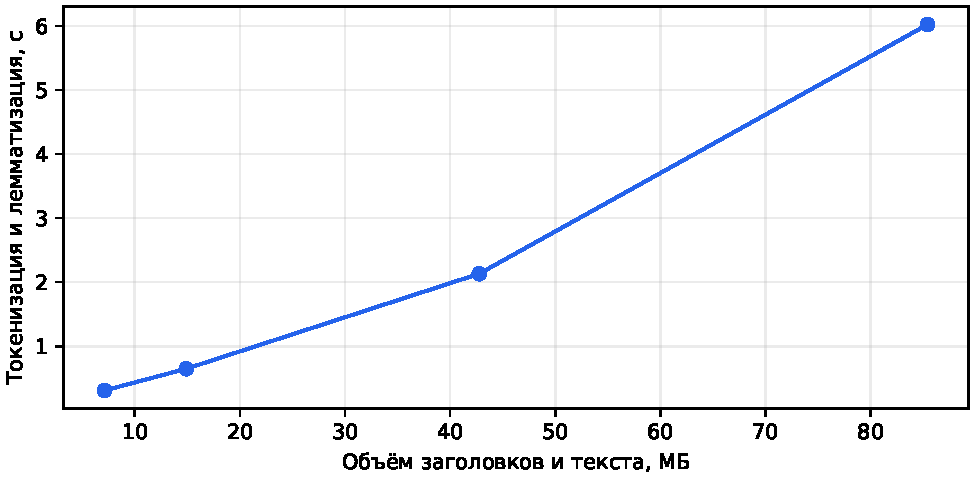
\includegraphics[width=.86\linewidth]{lab4/timing.pdf}
\caption{Зависимость времени обработки от объёма входного текста}
\end{figure}

Здесь КБ означает 1000 байт, МБ --- 1\,000\,000 байт. Нельзя утверждать,
что скорость оптимальна: для дальнейшей работы полезно сравнить упаковку
ключей и вариантов, локальность памяти и параллельную обработку документов.
Нужно учитывать и отдельную стоимость загрузки относительно короткого запроса.
Повторные сырые замеры сохранены; скорость зависит от фоновой нагрузки машины.

Приведённые замеры обработки относятся к исходному снимку
из \CorpusDocuments{} документов. Отдельный эксперимент ниже
использует индекс 478\,833 документов. Работа на миллионе документов
данными экспериментами не проверялась.

\subsection{Качество и ошибки поиска}

\begin{table}[htbp]
\centering
\begin{tabularx}{\linewidth}{@{}Xrrr@{}}
\toprule
Режим & $P@5$ & $Recall@5$ & $nDCG@5$\\
\midrule
\LabFourQualitySummary
\bottomrule
\end{tabularx}
\caption*{Средние значения на фиксированном диагностическом наборе заголовков}
\end{table}

\begin{table}[htbp]
\centering
\small
\begin{tabularx}{\linewidth}{@{}Xrrr@{}}
\toprule
Запрос & Токены & Леммы & С бонусом\\
\midrule
\LabFourQualityRows
\bottomrule
\end{tabularx}
\caption*{$nDCG@5$ по запросам; оценки относятся только к выбранному набору}
\end{table}

На запросах «обновления Nintendo», «обзоры гарнитур» и «reviews Witcher»
лемматизация позволяет найти заголовки с другой словоформой. При этом
она не переводит русский запрос в английский: пример с Minecraft
не получает все релевантные документы только за счёт морфологии.

Важный отрицательный пример --- \code{Windows}. Без лемматизации первые
пять результатов относятся к операционной системе, $nDCG@5=1$.
После нормализации \code{Windows} и \code{windows} сближаются с
\code{window}. В выдачу попадают публикации про \emph{release windows},
то есть сроки выхода игр, а не ОС. Из-за равенства базовых оценок и порядка ID
значение падает примерно до 0,553. Бонус за исходное точное совпадение
возвращает пять заголовков про Windows и значение 1. На остальных запросах
этого набора ухудшения от бонуса не наблюдалось; это не гарантия для всех запросов.

В запросе \code{Windows 10} дополнительный контекст уже отсекает эти
ложные кандидаты. У \code{Saw} остаются другие трудности: название франшизы
совпадает с обычным английским словом, а притяжательная форма с апострофом
сохраняется токенизатором и может не совпасть с запросом. Один бонус
не устраняет смысловую неоднозначность. Возможные дальнейшие улучшения ---
контекст, учёт названий и явные правила притяжательных форм с отдельной
проверкой качества. Словарное расширение всех вариантов повышает полноту,
но способно снизить точность.

Разметка, полные списки выдачи и метрики находятся в
\path{tests/fixtures/lab4_judgments.json}, \path{lab4/quality.json}
и локальном каталоге эксперимента. Результаты на 37 заголовках
характеризуют диагностическую выборку; репрезентативной оценкой
качества на всём корпусе они не являются.

\subsection{Сравнение на булевом индексе большого корпуса}

Дополнительный эксперимент выполнен на снимке из 478\,833 документов
с использованием индекса ЛР7 и поискового ядра ЛР8. Индексируются
заголовок и основной текст. Словоформы и леммы хранятся в двух
независимых пространствах терминов одного физического индекса;
ID и метаданные документов общие. В обоих режимах применяются
один разбор выражений и одинаковые операции над списками документов.

В режиме словоформ операнд после нормализации ищется непосредственно.
В режиме лемм документ при индексации включается в списки всех
различных разборов каждого слова. При поиске выполняется такое же
преобразование операндов, и списки альтернатив объединяются.
Таким образом, различие результатов определяется морфологическим
представлением, а не сменой правил булевых операций или состава корпуса.
Используется тот же двуязычный морфологический словарь.

\begin{table}[H]
\centering
\small
\begin{tabularx}{\linewidth}{@{}Xrr@{}}
\toprule
Запрос & Словоформы & Леммы\\
\midrule
Mimir AND has AND returned & 0 & 7\\
татуировки AND в AND видеоиграх & 8 & 62\\
игры AND doom & 2667 & 3703\\
игрой AND doom & 717 & 3703\\
\bottomrule
\end{tabularx}
\caption*{Точное число совпадений по заголовкам и основному тексту}
\end{table}

Запрос \code{Mimir AND has AND returned} не находит документов
при требовании точных словоформ и возвращает семь при лемматизации.
В выдаче появляется публикация о возвращении актёра, озвучивающего
Мимира в God of War (рис.~\ref{fig:mimir-surface}--\ref{fig:mimir-lemma}).
Это пример полезного совпадения между различными формами слов.
Слова запроса могут находиться в разных частях документа:
запрос не является цитатой, порядок и соседство слов не проверяются.

\begin{figure}[H]
\centering
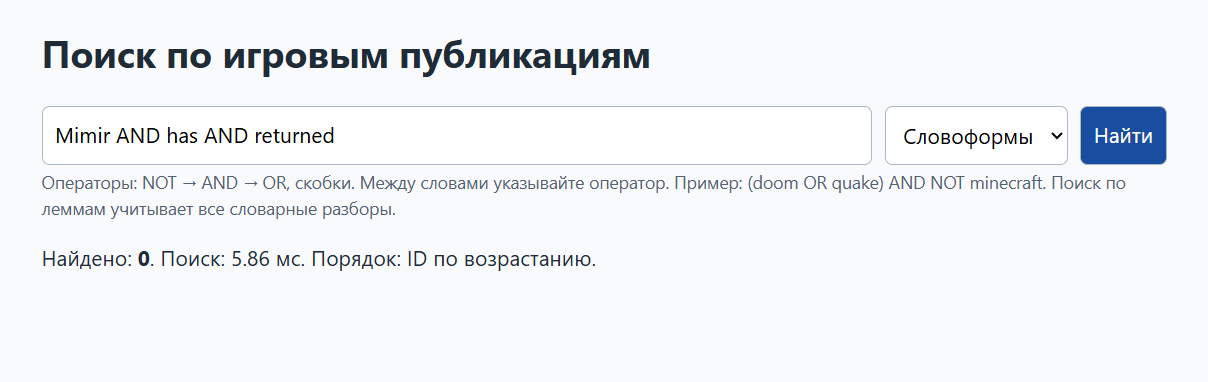
\includegraphics[width=\linewidth]{img/mimir_wordshapes.png}
\caption{Поиск запроса Mimir AND has AND returned по словоформам}
\label{fig:mimir-surface}
\end{figure}

\begin{figure}[H]
\centering
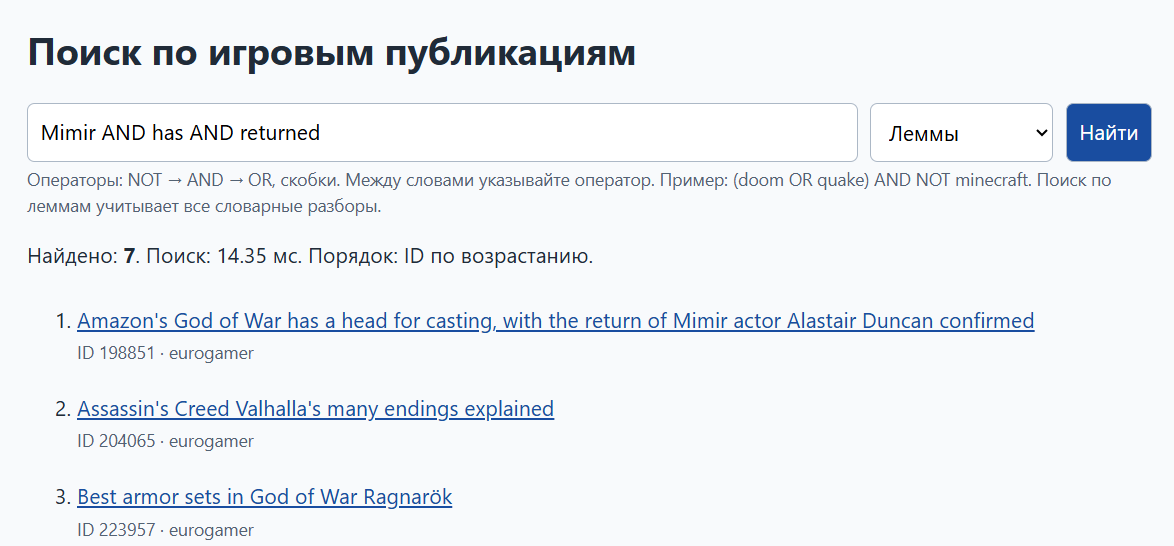
\includegraphics[width=\linewidth]{img/mimir_lemmas.png}
\caption{Тот же запрос в пространстве лемм}
\label{fig:mimir-lemma}
\end{figure}

В русском примере разные формы «игры» и «игрой» приводят
к одной лемме и дают одинаковое множество из 3703 документов
при дополнительном условии \code{doom}. Поиск словоформ возвращает
разные множества, поскольку требует конкретного написания.
Для запроса о татуировках число кандидатов увеличивается с 8 до 62.

Увеличение числа совпадений показывает расширение множества кандидатов,
но не заменяет измерения точности и полноты. Документы полного корпуса
в этом эксперименте не размечены; из семи результатов запроса о Мимире
не следует, что все семь релевантны. Порядок выдачи задан ID,
ранжирование и бонус за точное совпадение в булевом поиске не применяются.
Поэтому метрики диагностического ранжированного поиска выше
не переносятся на эти списки. Скриншоты показывают отдельные запуски;
время на них не является сравнительным замером производительности.

Сохранённые ответы с первыми документами, точные размеры множеств
и повторные измерения находятся в \path{lab4/boolean_comparison/}.
Запросы зафиксированы в \path{tests/fixtures/lab4_boolean_queries.txt}.

\subsection{Исходный код и воспроизводимость}

Инструкция подготовки словаря, сборки, запуска автотестов и эксперимента
приведена в \code{doc/lab4_run.md}. Исходной реализации соответствует адрес
\href{https://github.com/kirbasss/MAI-IR/tree/lab4}{github.com/kirbasss/MAI-IR/tree/lab4}.
Дополненный отчёт и эксперимент с булевым индексом находятся в ветке
\href{https://github.com/kirbasss/MAI-IR/tree/lab8}{lab8}.

\begin{figure}[htbp]
\centering
\begingroup
\hypersetup{urlcolor=black}
\qrcode[height=28mm]{https://github.com/kirbasss/MAI-IR/tree/lab4}
\endgroup
\caption{Ссылка на ветку лабораторной работы №4}
\end{figure}

\section{Вывод}

Реализована словарная лемматизация русских и английских слов
с сохранением неизвестных терминов и альтернативных разборов.
Собственная хеш-таблица обеспечивает обработку текста без выделения
памяти для каждого словарного токена. Модуль применён как к последовательной
обработке корпуса, так и к построению и поиску по инвертированному индексу.

На небольшом размеченном наборе поиск стал находить больше нужных заголовков,
но пример с Windows показал и обратную сторону: объединение словоформ
иногда добавляет посторонние результаты. Сохранение исходного слова и бонус
за точное совпадение улучшили результат на диагностическом наборе.
На индексе 478\,833 документов продемонстрировано расширение множества
кандидатов и одинаковый результат для разных форм одного русского слова.
Ограничения метода --- отсутствие контекстного снятия омонимии,
зависимость от покрытия словаря и возможное снижение точности.
Дальнейшая оценка требует расширения разметки релевантности;
применение бонуса за точное совпадение следует проверять
на запросах с названиями и неоднозначными словами.

\end{document}
